\chapter{Overview}
\label{ch:overview}

The main contribution of this dissertation is {\em a suite of solutions to make 
data-driven QoE optimization practical} -- one can substantially improve QoE 
by maintaining a global view of up-to-date network conditions based on the 
QoE information collected from many endpoints.
Our solutions achieve this through novel algorithm designs and system 
implementation that integrate machine learning techniques with domain-specific
insights.
%We  demonstrate that one can achieve substantial QoE improvement
%by utilizing measurement data already available to today's application 
%providers and integrating domain-specific insights with machine learning 
%techniques to make better real-time adaptation for client-side applications.
%In this chapter, we give an overview of our solutions, the key insight
%behind our solutions, and a perspective of how this solution compared 
%to prior efforts of Internet quality optimization and applying data-driven
%in the networking literature.

This chapter is organized as follows.
We begin with an overview of the envisioned 
architecture of data-driven QoE optimization, 
called {\em Data-Driven Networking} or {\em \ddn} (Section~\ref{sec:overview:arch}).
%some illustrative examples of how different applications 
%may benefit from \ddn, and perspective of how this solution compared 
%to prior work.
Then we discuss the algorithmic and architectural challenges of \ddn in 
Section~\ref{sec:overview:challenges}, motivate the unifying insights behind
our solutions in Section~\ref{sec:overview:unifying}, and finally describe
the key ideas of our solutions in Section~\ref{sec:overview:solutions}.
%describes a suite of solutions inspired by the insight to address \ddn's
%challenges in the context of Internet video and Internet telephony.


\section{Formalizing \ddn}
\label{sec:overview:arch}

We begin with a conceptual overview of the Data-Driven 
Networking (\ddn) paradigm (Section~\ref{subsec:overview:concept}),
and then put the \ddn approach in perspective of prior work 
(Section~\ref{subsec:overview:contrast}). We end with 
some illustrative examples of how different applications   
can benefit from \ddn (Section~\ref{subsec:overview:examples}).
%We end this section by identifying key factors that can impact 
%the potential benefits of \ddn.

\subsection{Conceptual Architecture}
\label{subsec:overview:concept}

\ddn is a new paradigm for designing the adaptation logic of 
end-to-end protocols (such as adaptive video streaming protocols). 
Unlike prior endpoint approaches, 
\ddn-based control loop is driven by real-time
{\em multi-session} (not single-session) view of 
{\em in-situ quality}~\cite{insitu} 
measurement (not active
measurements or indirect metrics), 
and {\em automatically tuned actuation algorithms} based
on data-driven insights (with little to no manual tuning).

A \ddn-enabled protocol has two additional components:
(a) the {\em client-side instrumentation} code which runs inside 
client-side application to measure client-perceived quality of 
each session and applies decisions made by \ddn; and 
(b) the {\em \ddn controller} which runs two loosely coupled steps:
\begin{enumerate}
\item Aggregate quality measurement from client-side 
instrumentation into a global view of up-to-date network conditions and 
some actionable insights.
\item Make control decisions based on the actionable insights, 
and send them to client-side instrumentation for execution.
\end{enumerate}

%Note that the \ddn paradigm is compatible to 
%the existing infrastructure operated by application 
%providers. For instance, many application providers 
%have already deployed client-side instrumentation to
%monitor client-side information in real-time and collect
%measurement for offline analytics (e.g.,~\cite{sigcomm11}).
%Many application providers also maintain a global control
%platforms (e.g.,~\cite{c3,via,footprint,chen2015end}) 
%where the \ddn controller can be implemented.

\ddn is aligned with several favorable technology trends, and can be 
readily deployed in the existing distribution infrastructures of Internet applications.
(1) Many application providers today have widely deployed client-side 
instrumentations that can collect real-time in-situ QoE data 
en masse from clients (e.g.,~\cite{sigcomm11,via,akamai-imc12,artizanetworks}). 
(2) Logically centralized control platforms are commonly deployed by many 
application providers (e.g., content providers~\cite{c3}, web services~\cite{footprint}) and CDN providers (e.g.,~\cite{chen2015end,mukerjee2015practical}).
(3) The emergence of large-scale data analytics platforms and cloud infrastructure 
provides the ability to extract insights efficiently from large corpses 
of data (e.g.,~\cite{spark}) and streams of updates 
(e.g.,~\cite{zaharia2013discretized}). 
%Such ability enables optimal decision making based on
%real-time data-driven predictions~\cite{velox-cidr}.


\begin{figure}[t!]
\centering
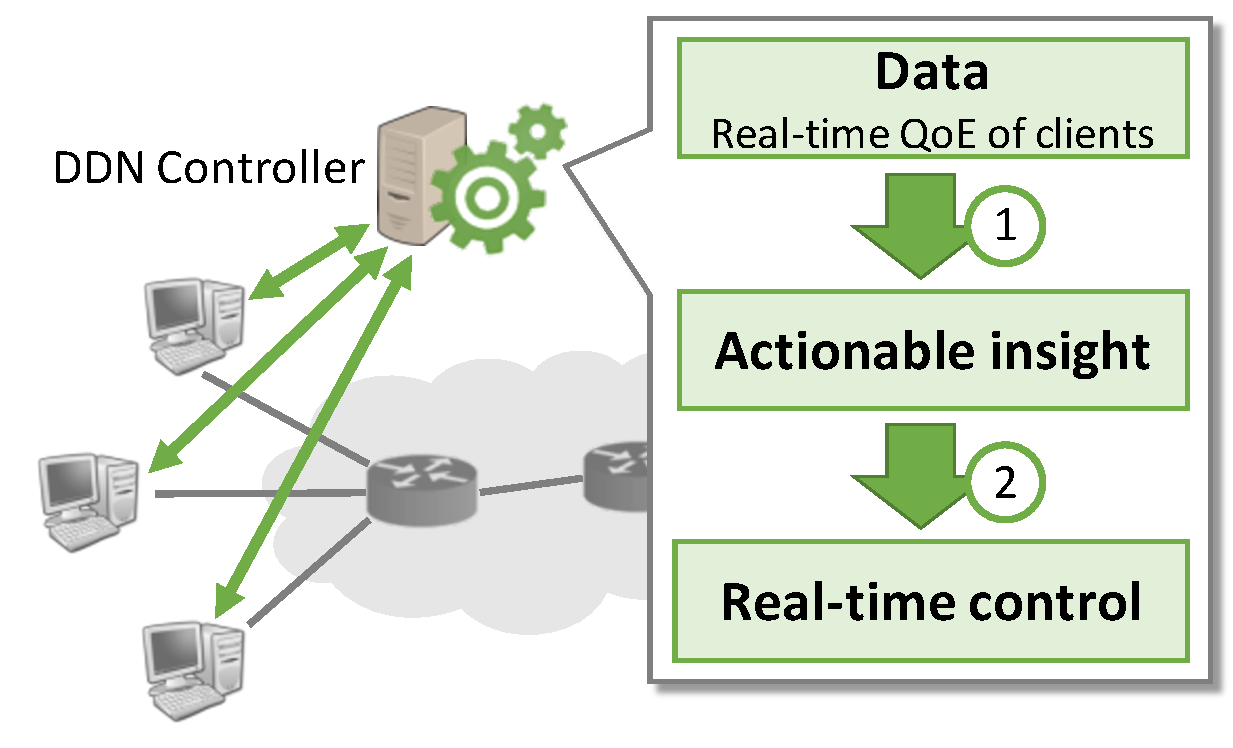
\includegraphics[width=0.6\textwidth]{figures/overview-ddn-arch.pdf}
%\vspace{-0.3cm}
\caption{Overview of the \ddn controller}
\label{fig:intro-contribution}
\end{figure}

\subsection{Contrast to Prior Work}
\label{subsec:overview:contrast}

The design choices of \ddn bear distinctive features compared to both prior work on quality
optimization and other applications of data-driven techniques in networking.

\mypara{Compared to prior work on quality optimization}
We use the taxonomy described in Section~\ref{sec:related:quality} to 
contrast the \ddn approach to QoE optimization with prior work.
Remember that there are two classes of prior solutions: in-network solutions that change 
in-network devices, and endpoint solutions that rely on endpoint adaptations.

%In Section~\ref{sec:related:quality}, we have classified
%prior work on quality optimization along two dimensions:
%where in the network (in-network vs. endpoints), and
%which level in the protocol stack (application vs. lower layers).
%Using this taxonomy, \ddn should be classified as an 
%endpoint solution operating in the application layer.

\begin{itemize}

\item Unlike prior endpoint solutions which use only single-endpoint 
information, decision making in \ddn is driven by QoE information of multiple endpoints. 
%The core argument of \ddn is that {\em it is feasible to
%maintain an accurate view of network conditions based on the QoE information
%collected from many endpoints}.
%Traditional end-to-end adaptation protocols (e.g., TCP/DASH) 
%is driven by what is observed by a single session. In contrast, 
By expanding the spatial scope of input information from the QoE of one 
single endpoint to that of multiple endpoints, 
\ddn addressing the endpoint approach's lacking of visibility to network conditions, 
while retaining its ethos that the decision is driven by user-perceived QoE at 
the application level.
%\ddn can predict the quality of a session if it uses certain decision, 
%as long as the decision has been used by some similar sessions.
\ddn is in spirit similar to seminal work from a decade agao (e.g., SPAND~\cite{spand}),
and our contribution lies in providing end-to-end solutions that combine 
the recent advances in large-scale data analytics and domain-specific insights
to make \ddn practical for today's applications.
%In short, \ddn retains the ethos of the endpoint approach, 
%while addressing its lack of
%visibility to network condition by leveraging an expended view 
%across many endpoints.

\item Unlike in-network solutions which rely on indirect signals on quality (e.g., acks 
or bandwidth), or active probes from a handful 
of vantage points (e.g., iPlane~\cite{iplaneosdi}), \ddn relies on in-situ QoE 
measurement to drive the adaptation; that is, what to be sensed matches
what to be optimized.
While in-situ quality data may compromise on the fidelity of 
individual measurement, they are far more efficient than 
alternatives in obtaining a panoramic and representative
 view of client-perceived quality from the growingly diverse platforms~\cite{insitu}.
%and the lack of fidelity can be compensated by harnessing the ``unreasonable effectiveness of data''~\cite{google-data}.
Relying solely on in-situ quality data also serves pragmatic 
purposes as many application providers today already have 
a vested interest in measuring user-perceived quality for 
various reasons~\cite{sigcomm-qoe-workshop}.

\end{itemize}





%To understand the contrast between  \ddn and traditional 
%control planes, it is useful to revisit the two logical steps 
%in the workflow of {\em any} control plane 
%(Figure~\ref{fig:sensing-actuation}):
%{\em sensing}, which gives the feedback data to control plane, 
%and {\em actuation}, which turns the feedback data to control decisions.
%\ddn radically departs from non-\ddn designs on both fronts 
%with two definitive features.

%(Table~\ref{tab:ddn} provides some examples to contrast between \ddn and non-\ddn designs.)

%\begin{itemize}
%\item {\em Multi-session view:} 
%Sensing of \ddn is based on multiple sessions, rather than single session. 
%Traditional end-to-end adaptation protocols (e.g., TCP/DASH) 
%is driven by what is observed by a single session. In contrast, 
%By extending the spatial scope of sensing to many sessions, 
%\ddn can predict the quality of a decision even before a session 
%actually uses it, as long as the decision has been used by 
%some similar sessions.
%
%\item {\em In-situ quality:}
%In \ddn, what to be ``sensed'' is exactly what to be optimized, i.e., quality perceived by all historical and ongoing sessions; 
%not indirect signals on quality (e.g., acks~\cite{jacobson1988congestion} or bandwidth~\cite{bwe}), or active probes from a handful of vantage points (e.g., iPlane~\cite{iplaneosdi}). 
%While in-situ quality data may compromise on the fidelity of individual measurement, they are far more efficient than alternatives in obtaining a panoramic and representative view of client-perceived quality from growingly diverse platforms~\cite{insitu}.
%%and the lack of fidelity can be compensated by harnessing the ``unreasonable effectiveness of data''~\cite{google-data}.
%Relying solely on in-situ quality data also serves pragmatic purposes as many application providers today already have a vested interest in measuring user-perceived quality for various reasons~\cite{sigcomm-qoe-workshop,sigcomm12,krishnan2013video}.
%
%%\item {\bf Automatically tuned control logic:}
%%To take full advantage of the enriched sensing data, actuation algorithms of \ddn should be dynamically tuned by data-driven insights with little to no manual configuration.
%%Unlike today's protocols where handpicked constants are used as key parameters (e.g., init\_cwnd and initial video bitrate), \ddn picks parameters~\cite{remy} and control logic~\cite{cs2p} based on quality feedback which indicates what suit the current operating condition the best.
%%Meanwhile, the \ddn control logic also needs to handle the {\em downside} of having more data (e.g., lack of fidelity in client-side measurement, and whether the data source is trustworthy) by harnessing the ``unreasonable effectiveness of data''~\cite{google-data}.
%
%\end{itemize}


%\begin{table}[t!]
%\centering
%\resizebox{0.6\textwidth}{!}{%
%\begin{tabular}{@{}cccc@{}}
%\toprule
%\textbf{} & \multicolumn{2}{c}{\textbf{Sensing}} & \textbf{Actuation} \\ \midrule
%\textbf{} & \textit{Multi-session} & \textit{In-situ quality} & \textit{Auto-tuned} \\ \midrule
%%\rowcolor[HTML]{FFFE65} 
%DDN & \Checkmark & \Checkmark & \Checkmark \\
%TCP AIMD~\cite{jacobson1988congestion} & $\times$ & $\times$ & $\times$ \\
%PCC~\cite{pcc} & $\times$ & \Checkmark & \Checkmark \\
%OSPF, BwE~\cite{bwe} & \Checkmark & $\times$ & $\times$ \\
%iPlane~\cite{iplaneosdi} & \Checkmark & $\times$ & NA \\
%RemyCC~\cite{remy} & $\times$ & $\times$ & \Checkmark \\ \bottomrule
%\end{tabular}%
%}
%\vspace{0.3cm}
%\caption{Difference of \ddn to non-\ddn strategies.}
%\label{tab:ddn}
%\end{table}

%\subsection{Contrast to Prior Work on Data-Driven Optimization}
\mypara{Compared to prior work on data-driven optimization in networking}
In the taxonomy of Section~\ref{sec:related:data}, \ddn belongs to the type 
(Section~\ref{subsec:related:data:type2}) in which decisions are driven by 
directly modeling their impact on the metric of interest (i.e., QoE).
%though \ddn can be applied to the first type (Section~\ref{subsec:related:data:type1}) 
%to find better configurations of existing logic.
%we have described two types
%of data-driven optimization in networked systems:
%better parameter setting, and better run-time decision making.
%Under this taxonomy, \ddn belongs to the second type, but with a 
The key distinction of \ddn is that the decisions are driven by real-time data 
from many different application sessions, rather than a single session as in
prior work. This difference has two profound implications.
%, from the perspective of data-driven paradigm.
(1) The input data of \ddn is much larger both in scale and scope, allowing 
\ddn to learn a more accurately model of the network conditions and make 
more informed decisions.
(2) The input data of \ddn is collected from concurrent and history sessions 
that have different session-level features (client-side, network-level, and server-side), 
so the \ddn decision logic must take into account the potentially complex 
relationship between these session-level features and QoE.


\subsection{Illustrative Examples of \ddn Benefits}
\label{subsec:overview:examples}

Several early applications of \ddn from prior work have shown 
tremendous promise of this new paradigm.
%how \ddn can be adapted to various use cases 
%to exploit their potential benefits. %(depicted in Figure~\ref{fig:early-examples}).

\mypara{CDN/bitrate selection for video}
The first example shows how a global view of video quality 
can optimize CDN and bitrate selection for individual video 
sessions. 
Video players today have the flexibility of streaming content 
from one of multiple CDNs and bitrates. However, with
only information on a single session, the current protocols 
always start with a default CDN and fixed (and conservative) 
bitrate, and gradually converge to a better bitrate and 
CDN by local trial-and-error strategies.
Given both performance of CDNs and client-side bandwidth 
have a substantial spatial diversity
  and temporal variability~\cite{sigcomm12}, there is a
remarkable room for improvement by dynamically mapping a 
session to the optimal CDN and bitrate with no trial-and-errors.
To exploit this opportunity, one can imagine a \ddn controller
that maps a video session  to the CDN and bitrate that has 
the best quality on similar sessions (e.g.,
those in the same AS and watching the same video content).
%Prior work~\cite{c3,cfa,cs2p} exploits this opportunity by mapping a video session 
% to the CDN and bitrate that has the best quality on similar sessions (e.g.,
%those in the same AS and watching the same video content); and it can reduce 
%the session duration spent on re-buffering by 50\% without lowering bitrates.


\mypara{Relay selection for Internet telephony}
The second example shows how VoIP quality can be improved by 
a \ddn controller that selects relay servers judiciously.
VoIP applications (e.g., Hangout and Skype) use relay servers 
for NAT traversal, where the selection of relay servers 
has traditionally been agnostic to real-time network conditions. 
But recent work has shown a
substantial room for improvement on call quality by selecting 
optimal relay servers for each
call~\cite{rewan-hotnets2015}. 
To exploit this opportunity, one can imagine a \ddn controller
that select near-optimal relay servers for individual Skype calls 
by identifying which relay has the best quality for similar calls 
(e.g., those between the same source and destination ASes 
on the same date).
%For instance, recent work~\cite{via} shows that one can select near-optimal relay servers for individual Skype calls by identifying which relay has the best quality for similar calls (e.g., those between the same source and destination ASes on the same date); 
%compared to non-relayed paths, this can alleviate 42\% of Skype calls whose quality is impacted by high packet loss rate ($>1.2$\%).
% by 42\%.


\mypara{Online service cluster selection}
The third example shows how the quality of online services 
(e.g., search engines) can be improved by a centralized 
control platform, which selects optimal proxies by consolidating
quality data of multiple applications and profiles of the infrastructure.
Recent work~\cite{footprint} takes the stance of a company who 
has the visibility and controllability over multiple applications as 
well as key infrastructure building blocks. 
By measuring end-to-end quality from clients and dynamically 
modeling the workload of network paths and servers, it can 
select proxies that reduce mean latency by 60\% and carry 2$\times$ 
more traffic, compared with a baseline that finds proxies by Anycast.

\mypara{File sharing}
Finally, file sharing applications (e.g., Dropbox) have
the flexibility to allow each client to fetch files~\cite{drago2012inside} 
from a chosen server or data center.  By using data-driven 
 approaches to predict the throughput between a client and
a server~\cite{cs2p,spand,zhang2001constancy}, we could 
potentially improve the QoE for these applications.


%\begin{figure}[t!]
%\centering
%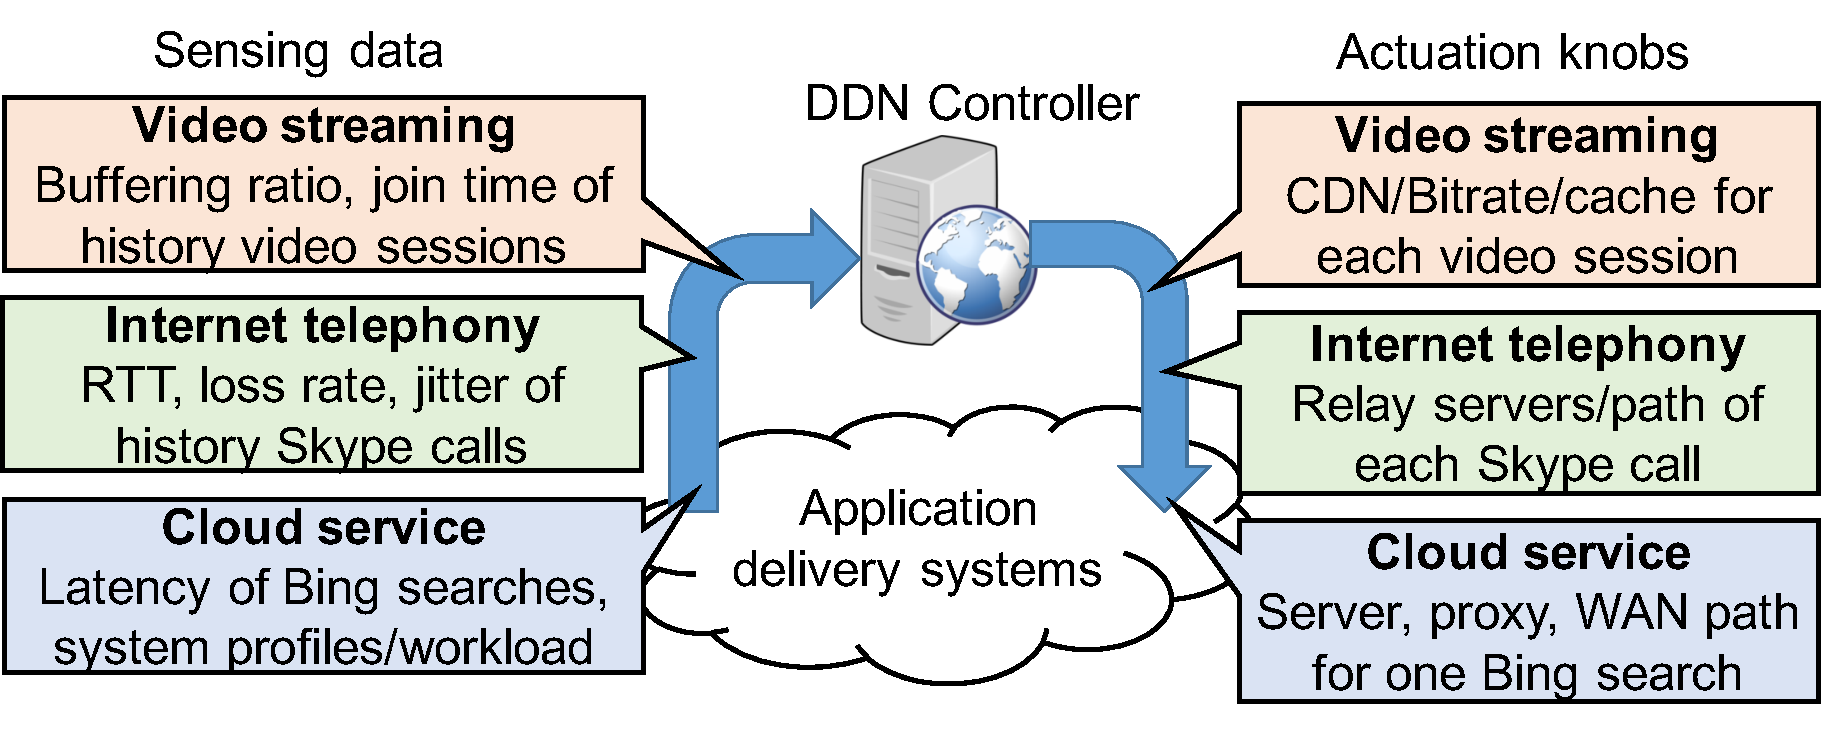
\includegraphics[width=0.8\textwidth]{figures/early-examples.pdf}
%%\vspace{-0.2cm}
%\caption{Examples of \ddn.}
%\label{fig:early-examples}
%\end{figure}



%\begin{figure}[t!]
%\centering
%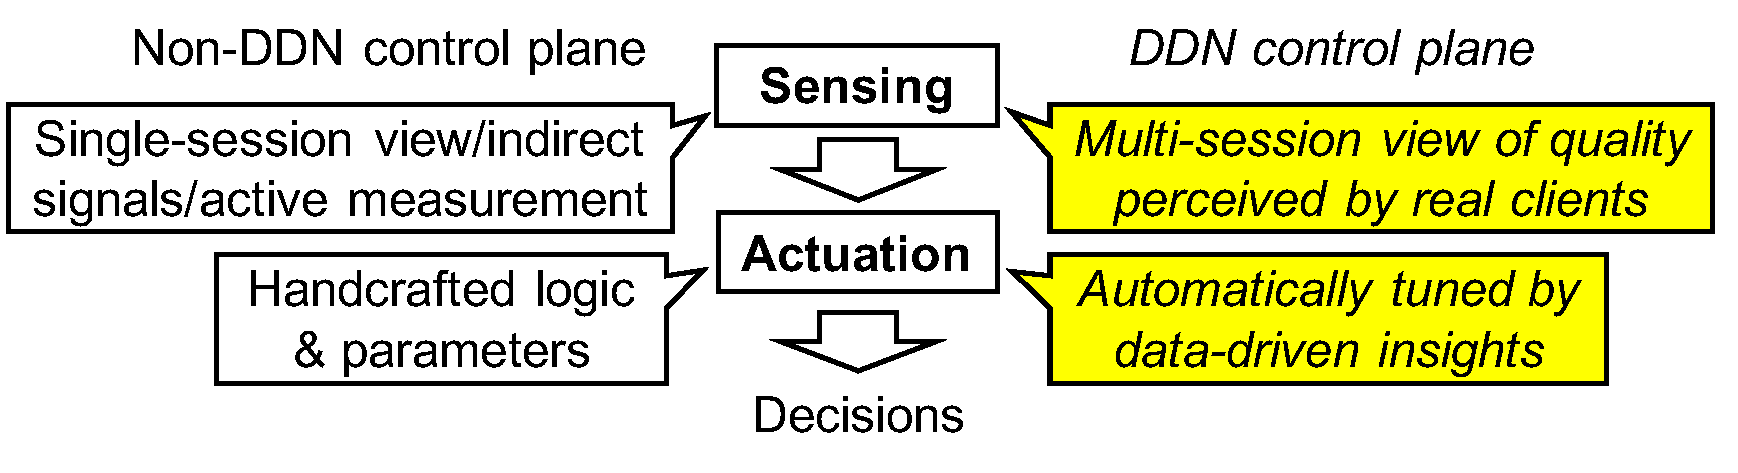
\includegraphics[width=0.8\textwidth]{figures/sensing-actuation.pdf}
%%\vspace{-0.7cm}
%\caption{\ddn control plane is fundamentally different to non-\ddn ones on both sensing and actuation.}
%\label{fig:sensing-actuation}
%\end{figure}



\section{Challenges of \ddn}
\label{sec:overview:challenges}

Despite its promise, \ddn has fundamental challenges that have to be addressed 
before we can unleash its full potential.
%This section describes two fundamental challenges 
%of \ddn and how they manifest themselves in various
%applications.
The next three sections present our roadmap (depicted in 
Figure~\ref{fig:overview-roadmap}) towards making \ddn practical. We start with
describing the high-level algorithmic and architectural challenges, and their 
manifestations we have seen in different applications.


\subsection{Need for Expressive Models}
\label{subsec:overview:challenge1}

The algorithmic objective of \ddn is to build a model that maps each 
session in the session-level feature space to the optimal decision in 
the decision space. 
%This is challenging for standard machine learning techniques,
%because such mapping is in a {\em high-dimensional} space.
At a high level, the challenges to build such a model stem from the complex 
relationships between session-level features, decisions, and QoE.
To address the challenge, we need an {\em expressive model} to express this complex 
relationship using the available measurement data.
We have seen two manifestations of the challenge of an expressive model.

\begin{itemize}

\item {\em High-dimensional relationship between session-level features and QoE:} 
The first illustration is the need to handle the complex relationship, both spatially 
and temporally, between video QoE and session-level features (Chapter~\ref{ch:cfa}).
This complex relationship has made it challenging to build an accurate video 
QoE prediction system, which could help to significantly improve video QoE.
%For instance, video 
%QoE can be substantially improved by dynamically selecting the optimal 
%CDN and bitrate using 
%based on a real-time global 
%view of network conditions.
%The key to realizing this promise is 
%a prediction model that can accurately predict the quality of any video session 
%based on QoE of similar sessions, if it were to use any CDN and bitrate.
%One challenge to practically build such prediction 
%model is that video QoE has complex relationship to 
%session-level features.
In particular, we observe a combinational effect where video QoE is affect by 
a specific combination of feature values, but does not appear to be correlated 
with any individual feature. We also observe that QoE of different sessions 
may be affected with different feature combinations. In addition to these spatial 
patterns, these QoE-determining factors (as well as QoE itself) may change
over time on timescales of several minutes. Therefore, an accurate QoE 
prediction model must be expressive enough to capture all these spatial and 
temporal complexities.

\item {\em Large decision spaces:}
The second illustration is the need to handle large decision spaces, especially in 
Internet telephony, where one needs to find a good relay path for each VoIP call
in a set of hundreds of relay points.
In addition, the performance of these relay paths could change on timescales 
of minutes.
%Prior work has shown that there is much room 
%for improving Skype quality by routing each 
%call through the optimal relay clusters in 
%the cloud.
%challenge
%However, identifying a close-to-optimal relay 
%in practice is very challenging, due to the sheer 
%number of possible relay paths (in hundreds) and 
%their dynamic performance (which could change 
%on timescales of minutes). 
%In addition, the number of calls different AS pairs
%follows a highly skewed distribution, so that
%in many AS pairs, the number of calls in each 
%hour is even less than the number of possible 
%relays.
Simply using geo-distance to reduce the decision spaces is suboptimal because 
low geo-distance to end users do not necessarily mean low latency and low packet 
loss rate which  have weak if any correlation with the geo-distance. Moreover, the 
best choice of relays depends  on locations of both caller and callee.
All these suggest a need to reduce the size of the mapping between
the client space and the decision space.

\end{itemize}



\begin{figure}[t!]
\centering
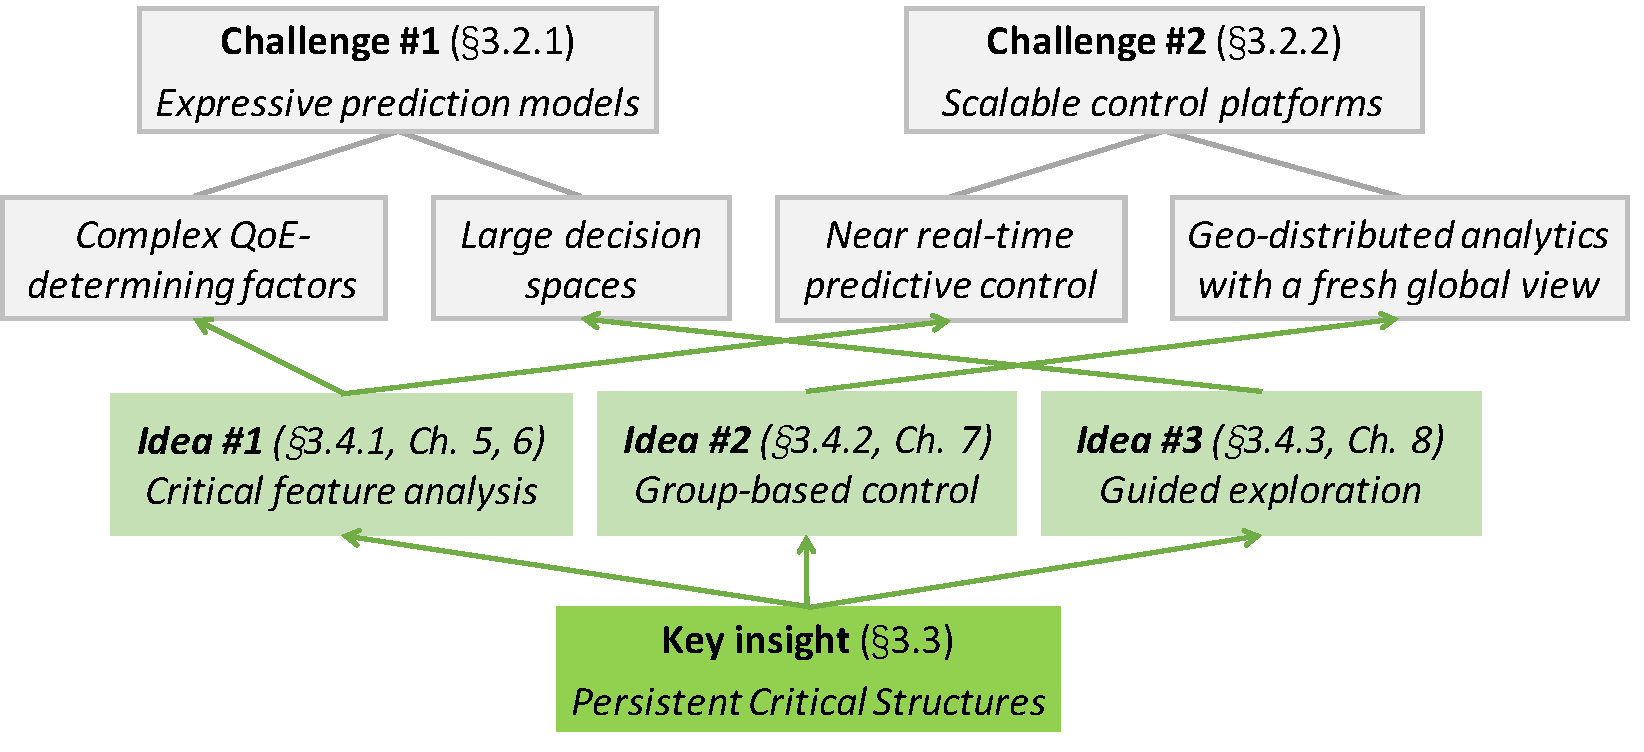
\includegraphics[width=0.88\textwidth]{figures/overview-roadmap.pdf}
%\vspace{-0.3cm}
\caption{
The technical roadmap of this dissertation towards making \ddn practical. We present three 
ideas to address the four manifestations of the high-level challenges of expressive prediction
models and scalable control platforms. The key enabling insight behinds our ideas is the 
persistent critical structures of QoE-determining factors. 
%The insight of persistent critical features inspires our three key ideas to 
%address four manifestations of \ddn's key algorithmic and architectural challenge.
}
\label{fig:overview-roadmap}
\end{figure}


%\begin{itemize}
%\item From data to insights requires expressive models
%\item Example 1: predictive model
%\item Example 2: reducing decision space
%\end{itemize}

\subsection{Need for Scalable Platforms}
\label{subsec:overview:challenge2}

The system design of \ddn should meet the following requirements:
the \ddn controller has to make control decisions 
in near real time based on fresh data from many
other geo-distributed clients, and serve the decisions 
to clients within low response time.
The key architectural challenge is how to strike a balance between 
three seemingly conflicting objectives: 
(1) {\em data freshness}, 
(2) {\em responsiveness to geo-distributed clients},
and (3) {\em global view}.
We have seen two manifestations of the challenge of a scalable platform.
%To make it more concrete, we again discuss two 
%manifestations of the challenge of a scalable platform.

\begin{itemize}
\item {\em Global view vs. data freshness:} 
%make decision with a fresh, global view of QoE of 
%many geo-distributed clients.
A practical issue of running the \ddn controller in the existing control platforms of 
application providers is that it is not clear how to maintain a fresh, global view of
measurement data from all sessions. 
These control platforms  typically consist of multiple geo-distributed frontend clusters 
and a centralized backend cluster. Each  session uploads its quality measurement 
to a nearby frontend, which  then updates the backend every tens of minutes 
to hours. While this design makes much sense for real-time per-session quality 
monitoring and offline analytics, none of which requires fresh, global data of all 
sessions, it is ill-suited to run the \ddn control logic in either the geo-distributed 
frontends (without global view) or the centralized backend (without fresh data).

%these control platforms  are not designed to collect
%fresh data from all sessions to the same physical data center, so that decisions can 
%be made based on a fresh, global view. Instead, each session uploads its
%quality measurement to a nearby geo-distributed frontend cluster, which 
%then syncs-up with the centralized backend cluster every tens of minutes
%to hours, because they are built for real-time 
%per-session quality monitoring and offline analytics, neither of which requires 
%a fresh and global data collected all clients, and it is costly to gather all data 
%into one cluster in real time.
%In this context, it seems not suitable to run the \ddn control logic in either 
%the geo-distributed frontends (without global view) or the centralized 
%backend (without fresh data).
%, so it would be 
%impractical to assume the decision-making algorithm 
%can run in a cluster which has a fresh, global view 
%of measurement data from all clients. 
%Besides, it is costly to gather all data into one cluster,
%because it requires to change the existing 
%data gathering procedure and to significantly increase 
%the communication overhead.
%Therefore, one challenge is to 
%perform geo-distributed analytics by striking a 
%balance between global view and data freshness.

\item {\em Near real-time predictive analytics:}
Even if we can gather real-time data to the same data center, it is still very 
challenging to run real-time analytics to predict the optimal decision in near 
real time, e.g., on a timescale of tens of seconds.
As mentioned in Section~\ref{subsec:overview:challenge1}, we need a large 
amount of data to update a high-dimensional model between session-level 
feature space and video QoE in near real-time (on timescales of tens of seconds). 
Our evaluation based on standard large-scale analytics platforms show that 
given the sheer volume of measurement data, it would take tens of minutes, 
a magnitude longer than needed, to update the model.

\end{itemize}

%\begin{itemize}
%\item From insights to real-time control requires scalable platform
%\item Example 1: Enabling complex real-time analytics
%\item Example 2: High responsiveness
%\end{itemize}


\section{Key Insight: Persistent Critical Structures of QoE-Determining Factors}
\label{sec:overview:unifying}

%\jc{add a formal definition and illustrative figures of persistent structures}

Our solutions to address these challenges integrate 
standard ML algorithms and 
systems with a key domain specific insight that Internet
%Before we show how to address these challenges, 
%it would be helpful to  first understand the key domain-specific insight that
%inspires our solution.
%One unifying theme behind these seemingly 
%independent ideas is to integrate 
%standard machine learning algorithms and 
%systems with the domain-specific insight that Internet 
applications have {\em persistent critical structures that help identify 
network sessions with similar QoE-determining factors, and that such 
structure tends to be persistent on timescales of 
at least tens of minutes}.
We now give the formal definition of persistent critical structures 
and how they intuitively help address \ddn's challenges.


\mypara{Formal definition}
Let us first formally describe \ddn as follows. 
In essence, \ddn is as a decision-making function 
$F:2^\mathbb{S}\times2^\mathbb{D}\times\mathbb{S}\times\mathbb{R}
\mapsto\mathbb{D}$, which takes as input a set of historical 
sessions $S\in2^\mathbb{S}$ whose 
QoE is already measured, a set of available decisions 
$D\in2^\mathbb{D}$, a new session $s\in\mathbb{S}$, and $s$'s timestamp
$t\in\mathbb{R}$,
and outputs a decision $d\in\mathbb{D}$ for session $s$.
Now, a {\em structure} is formally defined as a function 
$P:2^\mathbb{S}\times2^\mathbb{D}\times\mathbb{S}\times\mathbb{R}
\mapsto2^\mathbb{S}\times2^\mathbb{D}$,
which takes as input a set of historical  sessions $S\in2^\mathbb{S}$, 
a set of decisions $D\in2^\mathbb{D}$, and a session $s\in\mathbb{S}$, 
and the timestamp $t\in\mathbb{R}$, and outputs a pair of  subset of history sessions
$S'\subset{S}$ and a  subset of decisions $D'\subset{D}$.


\mypara{Key properties}
Persistent critical structures are a type of structures that have two following 
properties:

\begin{itemize}

\item {\em Criticality:} These structures identify (often small) subsets of history
sessions and decisions which are more critical than others history sessions 
or decisions in determining QoE; i.e.,
$F(S,D,s,t)=F(S',D',s,t)$, where $(S',D')=P(S,D,s,t)$. This essentially
means the \ddn control logic can make the same decisions by
only looking at the subset of relevant history sessions and decisions.

\item {\em Persistence:} These structures tend to persist on timescales of 
tens of minutes. This means in a time window $\Delta$ 
of  tens of minutes, the function $P$ is likely 
to find the same relevant history sessions and decisions,
i.e., $P(S,D,s,t)=P(S,D,s,t+\Delta)$.

\end{itemize}


\mypara{Illustrative examples}
These persistent critical structures of QoE-determining factors can 
manifest themselves in many forms.
For instance, if the QoE of a video session depends on
the server load (i.e., some decision-specific properties)
and client-side ASN (i.e., some session-level features), and such
dependency lasts for tens of minutes,
then it would be possible to identify the best decision for
the session by looking
at history sessions having in the same AS 
(instead of all history sessions), and only consider server with 
low load (instead of all possible decisions).

%\vspace{0.15cm}
%\noindent{\bf Why there are persistent critical structures?}
\mypara{Intuitively explanation of persistent critical structures}
The intuitive explanation of these persistent critical structures 
is that in networked systems and application delivery  systems, performance
bottlenecks are often persistent, and the persistent structures
can be viewed as ``manifestations'' of these bottlenecks in the space of 
session-level features and decision-specific properties--a session's QoE
only depend on history sessions and decisions 
experiencing the same bottleneck.
Such persistent bottlenecks can be found in many prior studies in the context
video streaming~\cite{cfa}, 
web service~\cite{footprint}, end-to-end
network performance~\cite{zhang2001constancy}.
They can also be viewed as a generalization of the persistent 
network congestions, which can be mathematically explained using queueing theory
(Chapter 6 of \cite{keshav2012mathematical}).
In Chapter~\ref{ch:measurement}, we will show evidence of these persistent
structures through an empirical structural analysis on  QoE
problems based on real datasets.

% For instance, video
%sessions with similar QoE from the same CDN/server tend to match on 
%client IP prefix~\cite{cfa,cs2p}. 
%Similarly, VoIP calls between the same ASes are likely to share the best
%relays~\cite{via},  and clients from  same /24 IP prefix will have
%similar web load time from the same edge proxy~\cite{footprint}.

%which takes as input a given set of historical 
%sessions $S\in2^\mathbb{S}$ and a new session $s\in\mathbb{S}$,
%and outputs a subset of history sessions $S'\subset{S}$; 
%and $L:2^\mathbb{D}\times\mathbb{S}\mapsto2^\mathbb{D}$, 
%which takes as input a given set of available decisions
%$D\in2^\mathbb{D}$ and a new session $s\in\mathbb{S}$,
%and outputs a subset of these decisions $D'\subset{D}$.


%For instance, the persistent critical features 
%(Section~\ref{subsec:overview:cfa}) can be
%viewed a kind of persistent structure which
%groups video sessions that match values on
%their critical features.
%The fact that there is a stable subset of 
%promising relay choices for each AS pair 
%(Section~\ref{subsec:overview:guided}) 
%can be viewed as another example of 
%persistent structure, where the structure
%is the subspace of the large decision space.


%\vspace{0.2cm}
%\noindent{\bf How intuitively persistent critical structures address the challenges?}
%\mypara{Why persistent critical structures are helpful}


\begin{figure}[t!]
\captionsetup[subfigure]{justification=centering,farskip=-1pt,captionskip=5pt}
\centering
%\hspace{-0.5cm}
\subfloat[Reducing session-level feature spaces.]
{
        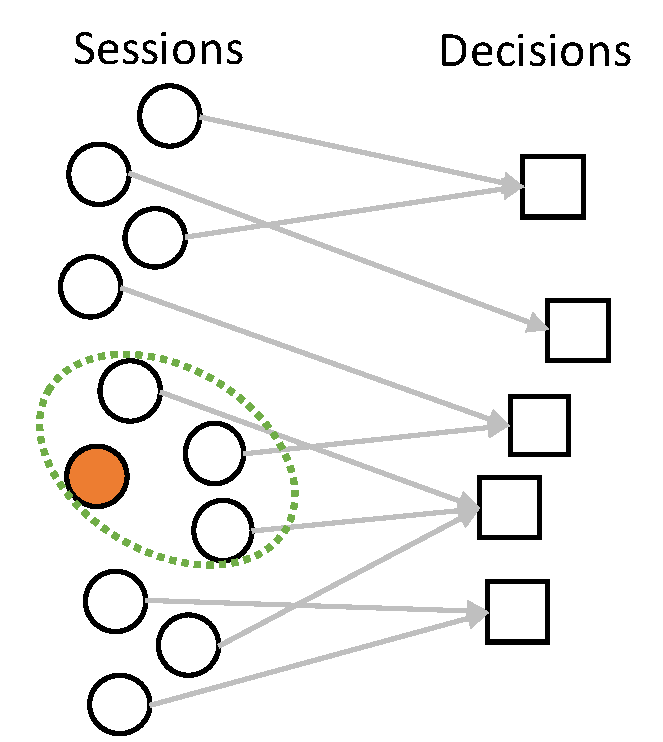
\includegraphics[width=0.33\textwidth]{figures/overview-idea-1.pdf}
        \label{subfig:overview-idea-1}
}
\subfloat[Reducing large decision spaces.]
{
        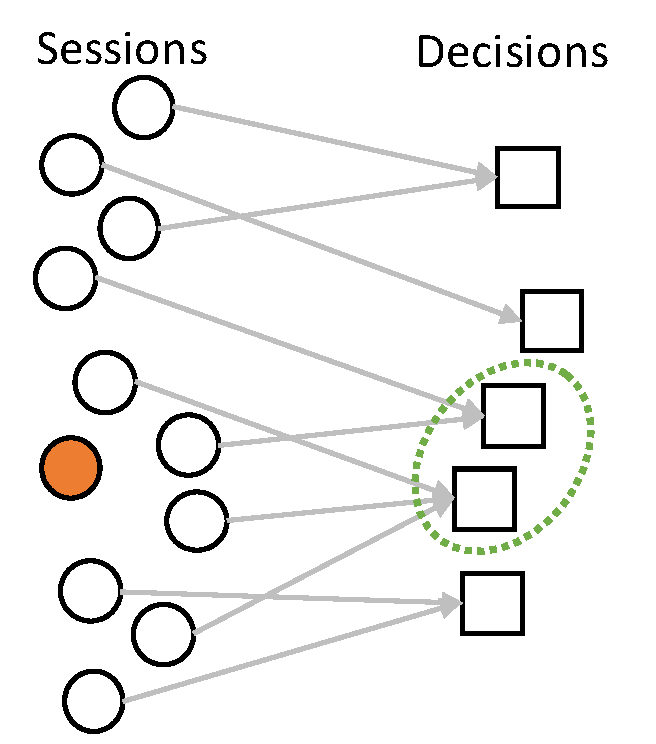
\includegraphics[width=0.33\textwidth]{figures/overview-idea-2.pdf}
        \label{subfig:overview-idea-2}
}
\subfloat[Decomposing the decision-making process.]
{
        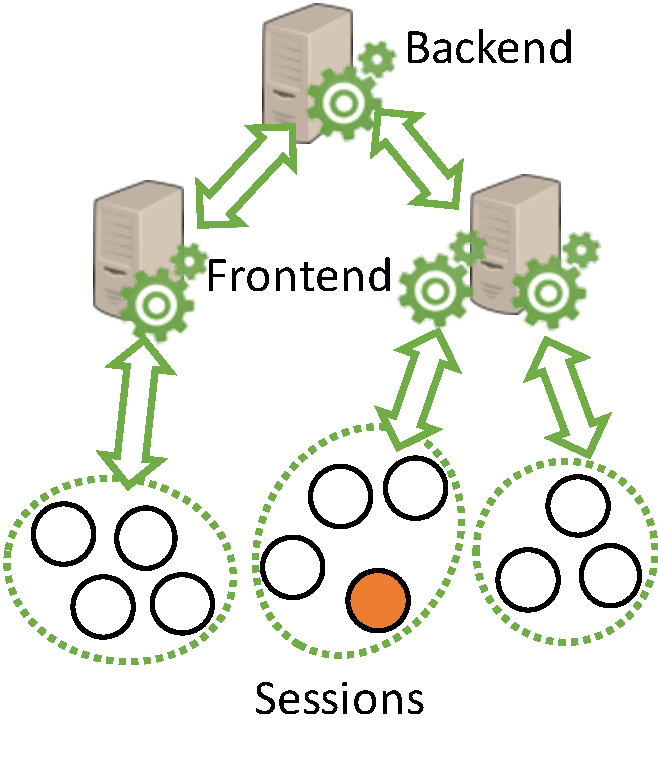
\includegraphics[width=0.33\textwidth]{figures/overview-idea-3.pdf}
        \label{subfig:overview-idea-3}
}
%\vspace{-0.2cm}
\caption{Illustrations of how persistent critical structures help to address challenges 
of \ddn. (Each application session (depicted as a circle) on the left is mapped to one 
of the available decisions (depicted as boxes) on the right. )}
\vspace{-0.1cm}
\label{fig:overview:ideas}
\end{figure}


\subsection{How Intuitively Persistent Critical Structures Address the Challenges?}
%Persistent critical structures are the key enabler behind our solutions of expressive 
%models and scalable control platform for \ddn. 
Here, we present an intuitive explanation of how persistent critical structures help to 
address challenges of \ddn (illustrated in Figure~\ref{fig:overview:ideas}).

%\begin{itemize}

\mypara{Reducing session-level feature spaces} 
One implication of the criticality property of these domain-specific structures is that 
the complex relationship between session-level features and QoE (the first manifestation 
of challenge of expressive models in Section~\ref{subsec:overview:challenge1}) can be 
expressed low dimensional models that can be maintained with limited available data.
%can be expressed by low dimensional models.
%This allows us to build models that focus on these  domain-specific structures, 
%which are expressive enough to capture the complex relations between 
%session-level features and decisions with limited available data.
To see this idea in action, let us consider the example of 
Figure~\ref{subfig:overview-idea-1},  in which we want to make the decision for a new 
session (the orange circle) based on the QoE measured by the history sessions 
(the white circles). It is not ideal to look at only the sessions that
match values on all features (e.g., IP prefix, location, device, content, network 
path, etc), which will leave too few matches.
%It is not scalable to use all history sessions to make 
%the decision in real time, and neither is it ideal to look at only the sessions that
%match values on all features (e.g., IP prefix, location, device, content, network 
%path, etc), which will leave too few matches.
As we will see, an illustration of persistent critical structures is that each session's 
QoE only depends on by a few critical features (rather than all features). Therefore, 
we can find many similar sessions by matching along the most relevant features. 
This idea resembles the ML techniques that leverage the ``locality'' in data to tackle 
curse of dimensionality~\cite{ml101}.

\mypara{Reducing large decision spaces} Another implication of the criticality property is that the large decision spaces 
(the second manifestation of challenge of expressive models in 
Section~\ref{subsec:overview:challenge1}) can be reduced to a subset of most promising 
decisions which can be explore efficiently by concurrent application sessions who share
the same characteristics. Figure~\ref{subfig:overview-idea-2} illustrates an example of this 
idea, where instead of exploring all decisions, it is sufficient to focus on a subset of 
decisions that are most likely to be the optimal one.


\mypara{Decomposing the decision-making process} 
In the context of network applications, the persistent critical structures often 
correlate with network locality (e.g., clients in the same IP prefix). This allows us to strike
a balance between global view and data freshness (Section~\ref{subsec:overview:challenge2}). 
The critical structures enable an effective decomposition of all sessions into {\em groups} of
similar sessions who share the persistent critical structure as well as the network locality. 
Figure~\ref{subfig:overview-idea-3} illustrates how such decomposition helps to strike
a balance between global view and data freshness. 
Since the sessions in the same group share network locality, their QoE measurement
will be sent to the same nearby frontend cluster. This suggests that in each group, we can 
use a decision-making logic that runs in the frontend cluster and only uses the information 
of these similar sessions. In this way, the decisions are effectively equivalent to using a 
fresh global view, because they are made with fresh data of the most relevant sessions.

\mypara{Learning the persistent critical structures from data} 
While the criticality of these persistent critical structures serves the key to addressing
many challenges of \ddn, it is so far unclear how to obtain these structures in the first place. 
The key to learn these structures lies in their persistence. 
Since these structures tend to persist on longer timescales than QoE itself does, we can learn 
these structures from more history data with an offline process separate from real-time decision 
making. Figure~\ref{subfig:overview-idea-3} illustrates the idea: we can run an algorithm in the 
backend cluster to discover the  persistent critical structures, because the 
backend cluster the measurement data of all clients, and although the data is slightly stale,
we found that it is still suitable to learn the slow-changing persistent critical structures.


%\end{itemize}





\section{Making \ddn Practical by Persistent Critical Structures}
\label{sec:overview:solutions}

The insight of persistent critical structures enables our key ideas 
(Figure~\ref{fig:overview-roadmap})  to address \ddn's challenges. 
%Figure~\ref{fig:overview-roadmap} summarizes the 
%the mapping between the challenges and the ideas.
%We conclude the section by discussing a unifying
%insight underlying these solutions.

%of 
%{\em persistent structures--there exist some structure
%(e.g., performance bottlenecks) that identifies 
%network sessions with 
%similar QoE-determining factors, and that such 
%structure tends to be persistent on timescales of 
%tens of minutes}.
%The term ``structure'' is broadly defined, and will 
%have specific meanings when we discuss it in 
%context.
%Next, we will briefly describe how the persistent
%structures 

\subsection{Critical Features Analysis}
\label{subsec:overview:cfa}

As we have seen, video QoE can be improved by
a prediction system that accurately predicts the QoE 
of a video session if it uses a certain CDN and bitrate.
The challenge is that this prediction system must be 
(a) expressive enough to capture complex relations 
between video quality and observed session features, 
and (b) capable of updating quality predictions in near 
real time.
We used several off-the-shelf machine learning 
techniques, such as random forests and SVM, but 
found they did not produce expected QoE improvements, 
because the long-term historical data is too coarse grained 
for these algorithms to capture the dynamics of video 
quality, while the short-term historical data is not sufficient 
for the algorithms to learn complex relations between 
video quality and observed session features.

Our solution leverages an instantiation of persistent structures
in video streaming, called 
{\em persistent critical features: each video session has 
a small set of critical features that ultimately determines 
its video quality, and these critical features change much 
more slowly than video quality}. 
Let us consider a concrete example of such persistent 
critical features from~\cite{cfa}.
In a real-world incident, video sessions of Comcast
users in Baltimore who watched videos from Level3
CDN experienced high failure rate (VSF) for several
hours. The reason turned out
to be the overloaded local cluster serving Comcast
users in that area,
which can be characterized by three critical features: 
CDN (``Level3''), ASN (``Comcast'') and City (``Baltimore''),
and the correlation between the combination of these
feature values and high VSF persist for the whole
duration of this incident, even though the QoE
has fluctuated a lot during this period.

The insight of persistent critical features has inspired
a prediction model that captures complex QoE-determining 
factors and is amenable to scalable implementation.
Given a video session under prediction, the model 
identifies many similar sessions from a short-term 
history by matching only on its critical features,
thus capturing complex QoE determining factors
while avoiding curse of dimensionality.
The persistence of these critical features also naturally
enables decoupled implementation: 
we can learn these critical features from long-term historical 
data and update the models by short-term historical data 
in near real time to capturing quality fluctuation.


%%\paragraph{CFA: Improving QoE via Expressive Prediction Models.}
%%problem
%Delivering high QoE is crucial to the success of today's subscription-/ad-based business models for Internet video.
%There is substantial room for improving video QoE by dynamically selecting the optimal CDN (Content Delivery Network) and bitrate based on a real-time global view of network conditions~\cite{sigcomm-case,conext-shedding}.
%The key to realizing this promise is a {\em prediction oracle} that can accurately predict the quality of a video client if it uses a certain CDN and bitrate.
%%challenge
%The challenge is that this prediction system must be (a) expressive enough to capture complex relations between video quality and observed session features, and (b) capable of updating quality predictions in near real time.
%We used several off-the-shelf machine learning techniques, such as random forests and SVM, but found they did not produce expected QoE improvements, because the long-term historical data is too coarse grained for these algorithms to capture the dynamics of video quality, while the short-term historical data is not sufficient for the algorithms to learn complex relations between video quality and observed session features.
%%these algorithms fail to capture the quality variability when trained with long-term history data, and they fail to identify the complex prediction models when trained with short-term history data.
%%Unfortunately, several seemingly natural solutions (e.g., simple machine learning approaches and network models) fail on one or both fronts.
%%insight
%My solution, CFA~\cite{cfa}, leverages the domain-specific insight of {\em persistent critical features}; each video session has a small set of critical features that ultimately determines its video quality, and these critical features change much more slowly than video quality~\cite{conext-shedding}. 
%%I present the design and implementation of CFA~\cite{cfa} to address these challenges. 
%%CFA is driven by the domain-specific insight of {\em persistent critical features}, that each video session has a subset of critical features that ultimately determines its video quality, and these critical features tend to be persistent on timescales of tens of minutes~\cite{conext-shedding}. 
%%solution
%This insight enables us to learn complex prediction models from long-term historical data (thus expressing complex relations between video quality and session features), and update the models by short-term historical data in near real time (thus capturing quality fluctuation as well).
%%Therefore, CFA can predict video quality more accurately than many machine learning algorithms, though CFA may not be as good in other prediction tasks.
%%result
%A real-world pilot deployment shows that CFA leads to non-trivial improvements in video quality, e.g., 32\% less buffering time than industry-standard algorithms.
%Our conversation with domain experts confirmed that these improvements are significant for content providers and can potentially translate into substantial benefits in revenues.
%An end-to-end implementation of CFA has been deployed and used by Conviva, a company that offers video quality optimization services to many premium content providers. 
%
%The insight of persistent critical features turns out to be more general; e.g., I have also applied the same insight to accurate prediction of TCP throughput~\cite{cs2p}, which leads to 11\% higher video bitrate than state-of-the-art adaptive bitrate players (e.g., Netflix players) with no extra buffering.


\subsection{Group-Based Control}
\label{subsec:overview:group}

While the predictive decision-making algorithm 
described above shows promising QoE improvement, 
it faces has two fundamental limitations.
(a) Casting the data-driven QoE optimization as a
prediction problem suffers from the many known 
biases such as incomplete visibility.
%A natural solution is to re-cast the problem
%as a real-time exploration and exploitation process,
%which however, is not trivial due to the fact that 
%measurement data of one client is useful only
%to the clients sharing the same QoE-determining
%factors.
(b) The prediction algorithm is not a geo-distributed one, 
so it requires a fresh and global view be maintained in
one cluster. Having a fresh and global view 
physically in the same cluster is, however, impractical 
because in many control platforms, measurement 
data are first collected in several geo-distributed frontend 
clusters each having a partial view of nearby clients,
and then periodically archived in a backend cluster
to form a global though slightly staled view.
A baseline approach is to run control logic in a 
single backend cluster with global data from frontend 
clusters, but this approach leads to non-trivial 
staleness of the global data and suboptimal decisions.


To overcome these limitations, we re-cast the 
data-driven QoE  optimization as a real-time 
exploration and exploitation process, and build 
a practical system to run it among all clients at 
scale. 
Our key insight is inspired by the criticality of persistent
structures -- {\em the clients that exhibit similar 
QoE behavior will have similar network-level 
features (e.g., same IP prefix), and thus their 
fresh data will likely be collected by the same 
frontend cluster.}
We see manifestations of this insight in many 
settings.
% When clients share certain location or IP prefix-related
%features, they are more likely to have the similar video QoE~\cite{cfa} and
%similar TCP throughput~\cite{cs2p,spand} at the same point of time. 
For instance, video sessions with similar QoE 
from the same CDN/server tend to match on 
client IP prefix~\cite{cfa,cs2p}. 
Similarly, VoIP calls between the same ASes 
are likely to share the best
relays~\cite{via},  and clients from  same /24 
IP prefix will have
similar web load time from the same edge 
proxy~\cite{footprint}.

This insight inspires the notion of {\em group-based 
control}, which enables the real-time global 
exploration-exploitation process by decomposing 
the process into subprocesses, each controlling 
a group of clients with similar context by
network locality and other key session-level features 
and running in the frontend cluster that has these 
clients' fresh data.
Since sessions within a group share network locality (e.g., 
in the same locations and IP prefixes), 
they are likely to be mapped to the same frontend cluster.
By running the per-group exploration-exploitation 
logic in this frontend cluster, we can update
decisions with fresh data from other sessions i
n the group received by this frontend cluster.


%%\mypara{\underline{\smash{Real-Time Exploration and Exploitation At Scale.}}}
%%\paragraph{Pytheas: Improving QoE via Exploration and Exploitation at Scale.}
%%\mypara{Real-Time Exploration and Exploitation at Scale:}
%%problem
%While formulating data-driven QoE optimization as a prediction 
%problem has shown promising QoE improvement (e.g., CFA), 
%it is necessarily incomplete, as 
%it suffers from many known biases such as incomplete visibility, 
%and cannot respond to sudden changes such as flash crowds.
%Drawing a parallel from machine learning (e.g., ad recommendation), I argued that data-driven QoE optimization should instead be cast as a {\em real-time exploration and exploitation} process. % rather than as a prediction problem. 
%Measurement collection (exploration) could be informed by decision making (exploitation) to explore the decisions with less data, thus addressing the shortcomings of the prediction-based formulation.
%This new formulation is complementary to CFA, since CFA's prediction model can be reused to capture similarities among clients.
%%challenge
%While many exploration-and-exploitation algorithms are available, enabling these algorithms in networking introduces an architectural challenge: we need a {\em scalable control platform} to update decisions with fresh global data from clients, despite data coming from a variety of geo-distributed front-end clusters, each with only a partial view of the clients.
%%The key challenge of real-time exploration and exploitation in networking is how to update decisions in real-time for millions of geo-distributed clients using their fresh measurement data.
%%insight
%A baseline approach is to run control logic in a single back-end cluster with global data from front-end clusters, but this approach leads to non-trivial staleness of the global data and suboptimal decisions.
%I take an alternative approach; the control logic is run by geo-distributed front-end clusters which have fresh data, rather than the back-end cluster.
%The intuition is that the clients that exhibit similar QoE behavior will have similar network-level features (e.g., same IP prefix), and thus their fresh data will likely be collected by the same front-end cluster.
%%While the challenge might be intractable in a general setting, it
%%I address the challenge by the insight that network application sessions sharing the same {\em network- and application-level features} intuitively exhibit similar QoE behavior across different possible decisions.
%%solution
%Inspired by this insight, {Pytheas}~\cite{pytheas} uses the concept of {\em group-based exploration and exploitation}, which 
%%The key idea is to decompose the global exploration and exploitation process of all clients into processes within groups of similar clients and run these per-group processes in geo-distributed front-end clusters which are close to clients and have their fresh data.
%%The key idea is to decompose the global exploration and exploitation process into subprocesses of similar clients, and run each subprocess by the front-end cluster that is close to its clients and has their fresh data.
%decomposes the global exploration and exploitation process into subprocesses, each controlling a group of similar clients and running in the front-end cluster that has these clients' fresh data.
%%with both client-closeness and data-freshness.
%%result
%Using an end-to-end implementation in CloudLab, I show that compared to a state-of-the-art prediction-based system, Pytheas improves the average video QoE by up to 31\% and the 90th percentile QoE by 78\%.
%Pytheas is an open source project that enables application providers to deploy the proposed architecture at scale within their existing infrastructure. 


\subsection{Guided Exploration}
\label{subsec:overview:guided}

To make data-driven QoE optimization practical in Internet telephony,
we have to address an additional challenge that it has a 
large decision space of relay choices, so there 
are usually not enough VoIP calls to reliably estimate 
the dynamic network performance between each 
AS pair.

The key insight to address this challenge is  another
illustration of persistent structure --
{\em the stability of promising relay choices: for each pair of 
caller AS and callee AS, there is a small and 
stable subset of relays that almost always 
contains the best relay}. 
This insight has two implications: 
(1) because this subset of relays is stable, 
it can be learned from history; and 
(2) because this subset has only a few relays 
(less than five), it can be explored efficiently 
even with limited data.
Inspired by this insight, we develop a relay selection 
system that achieved close-to-optimal quality 
using the concept of {\em guided exploration}. 
The idea is to learn a small set of promising relays 
for each AS pair based on long-term (e.g., daily) 
historical data, and explore these relays using most
calls in real time.

%%\mypara{\underline{\smash{Reducing Large Decision Space.}}} 
%%\paragraph{VIA: Improving QoE in the Face of Large Decision Spaces.} 
%%\mypara{Reducing Large Decision Space:}
%%problem
%In the first large-scale study on Internet telephony quality, I found that a substantial fraction of Skype calls suffer from poor network performance, and that there is much room for improving Skype quality by routing each call through the optimal relay clusters in Microsoft's cloud.
%%challenge
%However, identifying a close-to-optimal relay in practice is very challenging, due to the sheer number of possible relay paths (in hundreds) and their dynamic performance (which could change on timescales of minutes). 
%Neither prediction-based methods (e.g., CFA) nor those based on exploration and exploitation (e.g., Pytheas) suffice to handle such a large decision space.
%%insight
%The key insight to address this challenge is that, for each pair of caller ISP and callee ISP, there is a {\em small and stable subset} of relays that almost always contains the best relay. 
%This insight has two implications: (1) because this subset of relays is stable, it can be learned from history; and (2) because this subset has only a few relays (less than five), it can be explored efficiently even with limited data.
%%the large decision space can be narrowed down to a {\em small subset} of relays that almost always contains the best relay, and such pruning can be learned from the historical data, because this set of most promising relays tends to be {\em persistent}.
%%solution
%Inspired by these intuitions, I developed {VIA}~\cite{via}, a relay selection system that achieved close-to-optimal quality using the concept of {\em guided exploration}. The idea is to learn a small set of promising relays for each ISP pair based on long-term (e.g., daily) historical data, and explore these relays using most calls in real time.
%%result
%Trace-driven analysis and a small-scale deployment shows that VIA cuts the incidence of poor network conditions for calls by 45\% (and for some countries and ISPs by over 80\%) compared to today's Skype quality.
%VIA has been used in Microsoft internal deployment with real Skype users, and is in the process of being fully deployed. 
%VIA was also used by Microsoft to identify the countries and ISPs where Skype quality can benefit the most if relaying services are deployed.
%%VIA is also used to identify the countries and ISPs where Skype quality can benefit the most from Microsoft relaying services.


%\subsection{How Persistent Structures Are Used}
 


\section{Summary}

In this section, we have discussed the advantages
of \ddn over prior approaches. 
In particular, as an application-level endpoint 
approach, \ddn enjoys the advantage of direct 
access to user-perceived QoE, and at the same
time, compensates the limited insight to network 
conditions by consolidating real-time measurement
from many endpoints, thus achieving the best world
of both endpoint solutions and in-network solutions.

We have also presented an overview of our solutions
to address \ddn's technical challenges--the need for 
expressive models and scalable systems. 
In particular, there are the three key ideas underlying 
our solutions: 
(1) critical feature analysis to enable an expressive 
QoE prediction model, 
(2) group-based control to enable real-time 
exploration-exploitation process at scale, and
(3) guided exploration to handle the large 
decision spaces in Internet telephony.
Finally, we summarize the section by distilling 
a unifying insight from these 
ideas--\ddn can be made practical by integrating
machine learning with the insight that there are 
persistent domain-specific structures.







